%\documentclass{standalone}
%\usepackage{tikz}
%\usetikzlibrary{patterns,plotmarks}
%\begin{document}
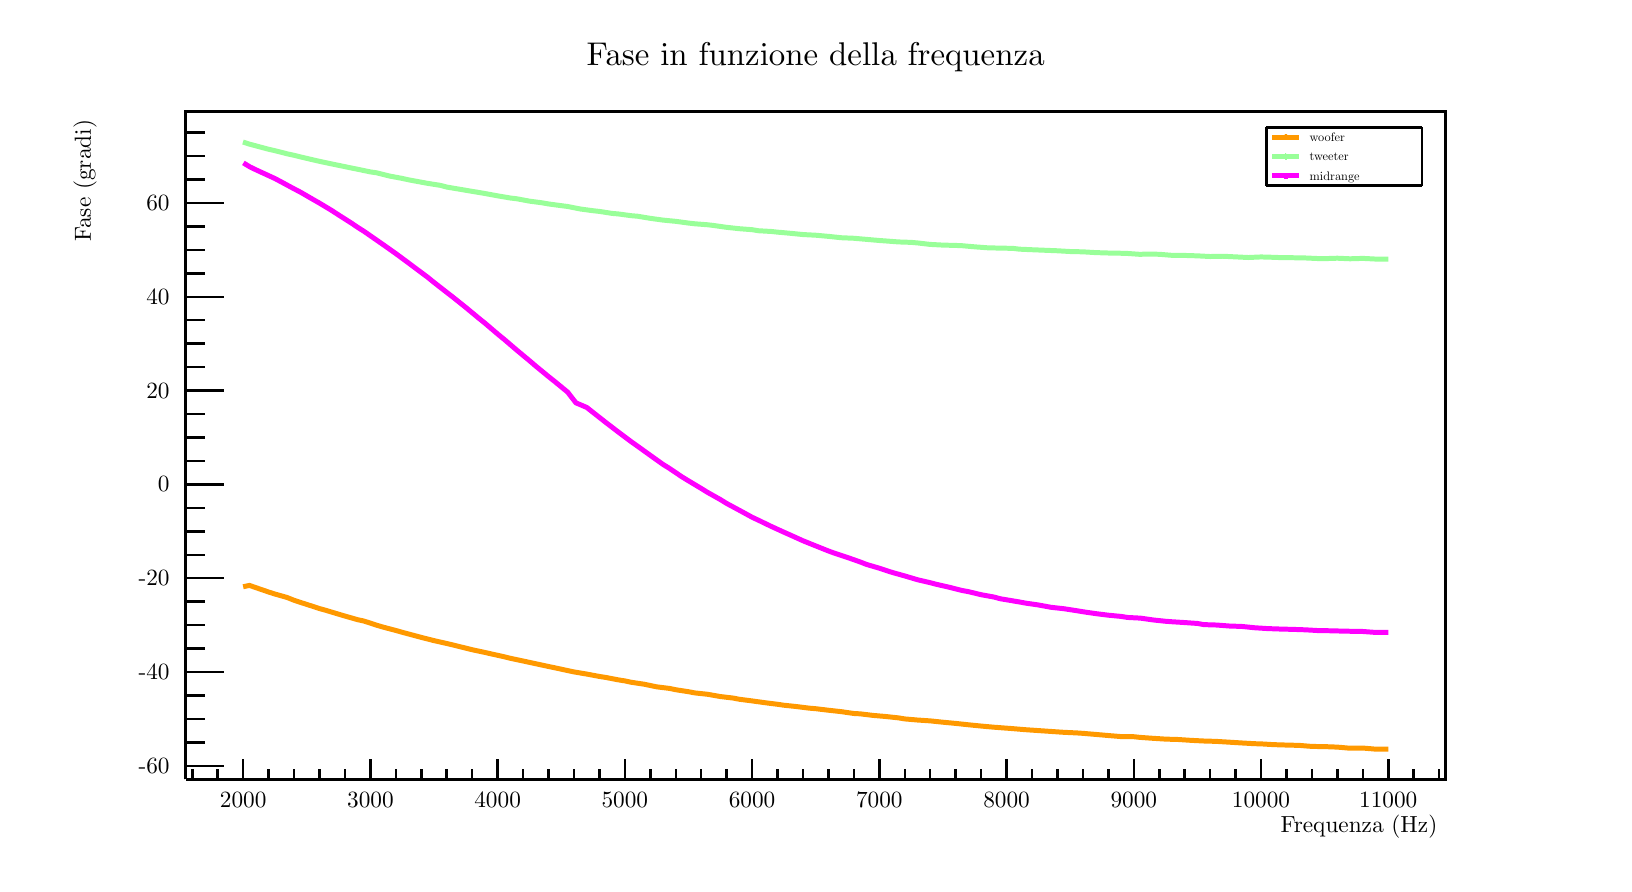
\begin{tikzpicture}
\def\CheckTikzLibraryLoaded#1{ \ifcsname tikz@library@#1@loaded\endcsname \else \PackageWarning{tikz}{usetikzlibrary{#1} is missing in the preamble.} \fi }
\CheckTikzLibraryLoaded{patterns}
\CheckTikzLibraryLoaded{plotmarks}
\pgfdeclareplotmark{cross} {
\pgfpathmoveto{\pgfpoint{-0.3\pgfplotmarksize}{\pgfplotmarksize}}
\pgfpathlineto{\pgfpoint{+0.3\pgfplotmarksize}{\pgfplotmarksize}}
\pgfpathlineto{\pgfpoint{+0.3\pgfplotmarksize}{0.3\pgfplotmarksize}}
\pgfpathlineto{\pgfpoint{+1\pgfplotmarksize}{0.3\pgfplotmarksize}}
\pgfpathlineto{\pgfpoint{+1\pgfplotmarksize}{-0.3\pgfplotmarksize}}
\pgfpathlineto{\pgfpoint{+0.3\pgfplotmarksize}{-0.3\pgfplotmarksize}}
\pgfpathlineto{\pgfpoint{+0.3\pgfplotmarksize}{-1.\pgfplotmarksize}}
\pgfpathlineto{\pgfpoint{-0.3\pgfplotmarksize}{-1.\pgfplotmarksize}}
\pgfpathlineto{\pgfpoint{-0.3\pgfplotmarksize}{-0.3\pgfplotmarksize}}
\pgfpathlineto{\pgfpoint{-1.\pgfplotmarksize}{-0.3\pgfplotmarksize}}
\pgfpathlineto{\pgfpoint{-1.\pgfplotmarksize}{0.3\pgfplotmarksize}}
\pgfpathlineto{\pgfpoint{-0.3\pgfplotmarksize}{0.3\pgfplotmarksize}}
\pgfpathclose
\pgfusepathqstroke
}
\pgfdeclareplotmark{cross*} {
\pgfpathmoveto{\pgfpoint{-0.3\pgfplotmarksize}{\pgfplotmarksize}}
\pgfpathlineto{\pgfpoint{+0.3\pgfplotmarksize}{\pgfplotmarksize}}
\pgfpathlineto{\pgfpoint{+0.3\pgfplotmarksize}{0.3\pgfplotmarksize}}
\pgfpathlineto{\pgfpoint{+1\pgfplotmarksize}{0.3\pgfplotmarksize}}
\pgfpathlineto{\pgfpoint{+1\pgfplotmarksize}{-0.3\pgfplotmarksize}}
\pgfpathlineto{\pgfpoint{+0.3\pgfplotmarksize}{-0.3\pgfplotmarksize}}
\pgfpathlineto{\pgfpoint{+0.3\pgfplotmarksize}{-1.\pgfplotmarksize}}
\pgfpathlineto{\pgfpoint{-0.3\pgfplotmarksize}{-1.\pgfplotmarksize}}
\pgfpathlineto{\pgfpoint{-0.3\pgfplotmarksize}{-0.3\pgfplotmarksize}}
\pgfpathlineto{\pgfpoint{-1.\pgfplotmarksize}{-0.3\pgfplotmarksize}}
\pgfpathlineto{\pgfpoint{-1.\pgfplotmarksize}{0.3\pgfplotmarksize}}
\pgfpathlineto{\pgfpoint{-0.3\pgfplotmarksize}{0.3\pgfplotmarksize}}
\pgfpathclose
\pgfusepathqfillstroke
}
\pgfdeclareplotmark{newstar} {
\pgfpathmoveto{\pgfqpoint{0pt}{\pgfplotmarksize}}
\pgfpathlineto{\pgfqpointpolar{44}{0.5\pgfplotmarksize}}
\pgfpathlineto{\pgfqpointpolar{18}{\pgfplotmarksize}}
\pgfpathlineto{\pgfqpointpolar{-20}{0.5\pgfplotmarksize}}
\pgfpathlineto{\pgfqpointpolar{-54}{\pgfplotmarksize}}
\pgfpathlineto{\pgfqpointpolar{-90}{0.5\pgfplotmarksize}}
\pgfpathlineto{\pgfqpointpolar{234}{\pgfplotmarksize}}
\pgfpathlineto{\pgfqpointpolar{198}{0.5\pgfplotmarksize}}
\pgfpathlineto{\pgfqpointpolar{162}{\pgfplotmarksize}}
\pgfpathlineto{\pgfqpointpolar{134}{0.5\pgfplotmarksize}}
\pgfpathclose
\pgfusepathqstroke
}
\pgfdeclareplotmark{newstar*} {
\pgfpathmoveto{\pgfqpoint{0pt}{\pgfplotmarksize}}
\pgfpathlineto{\pgfqpointpolar{44}{0.5\pgfplotmarksize}}
\pgfpathlineto{\pgfqpointpolar{18}{\pgfplotmarksize}}
\pgfpathlineto{\pgfqpointpolar{-20}{0.5\pgfplotmarksize}}
\pgfpathlineto{\pgfqpointpolar{-54}{\pgfplotmarksize}}
\pgfpathlineto{\pgfqpointpolar{-90}{0.5\pgfplotmarksize}}
\pgfpathlineto{\pgfqpointpolar{234}{\pgfplotmarksize}}
\pgfpathlineto{\pgfqpointpolar{198}{0.5\pgfplotmarksize}}
\pgfpathlineto{\pgfqpointpolar{162}{\pgfplotmarksize}}
\pgfpathlineto{\pgfqpointpolar{134}{0.5\pgfplotmarksize}}
\pgfpathclose
\pgfusepathqfillstroke
}
\definecolor{c}{rgb}{1,1,1};
\draw [color=c, fill=c] (0,0) rectangle (20,10.6013);
\draw [color=c, fill=c] (2,1.06013) rectangle (18,9.5412);
\definecolor{c}{rgb}{0,0,0};
\draw [c,line width=0.9] (2,1.06013) -- (2,9.5412) -- (18,9.5412) -- (18,1.06013) -- (2,1.06013);
\definecolor{c}{rgb}{1,1,1};
\draw [color=c, fill=c] (2,1.06013) rectangle (18,9.5412);
\definecolor{c}{rgb}{0,0,0};
\draw [c,line width=0.9] (2,1.06013) -- (2,9.5412) -- (18,9.5412) -- (18,1.06013) -- (2,1.06013);
\draw [c,line width=0.9] (2,1.06013) -- (18,1.06013);
\draw [c,line width=0.9] (2.72961,1.31457) -- (2.72961,1.06013);
\draw [c,line width=0.9] (3.05279,1.18735) -- (3.05279,1.06013);
\draw [c,line width=0.9] (3.37596,1.18735) -- (3.37596,1.06013);
\draw [c,line width=0.9] (3.69914,1.18735) -- (3.69914,1.06013);
\draw [c,line width=0.9] (4.02231,1.18735) -- (4.02231,1.06013);
\draw [c,line width=0.9] (4.34549,1.31457) -- (4.34549,1.06013);
\draw [c,line width=0.9] (4.66866,1.18735) -- (4.66866,1.06013);
\draw [c,line width=0.9] (4.99184,1.18735) -- (4.99184,1.06013);
\draw [c,line width=0.9] (5.31502,1.18735) -- (5.31502,1.06013);
\draw [c,line width=0.9] (5.63819,1.18735) -- (5.63819,1.06013);
\draw [c,line width=0.9] (5.96137,1.31457) -- (5.96137,1.06013);
\draw [c,line width=0.9] (6.28454,1.18735) -- (6.28454,1.06013);
\draw [c,line width=0.9] (6.60772,1.18735) -- (6.60772,1.06013);
\draw [c,line width=0.9] (6.93089,1.18735) -- (6.93089,1.06013);
\draw [c,line width=0.9] (7.25407,1.18735) -- (7.25407,1.06013);
\draw [c,line width=0.9] (7.57724,1.31457) -- (7.57724,1.06013);
\draw [c,line width=0.9] (7.90042,1.18735) -- (7.90042,1.06013);
\draw [c,line width=0.9] (8.2236,1.18735) -- (8.2236,1.06013);
\draw [c,line width=0.9] (8.54677,1.18735) -- (8.54677,1.06013);
\draw [c,line width=0.9] (8.86995,1.18735) -- (8.86995,1.06013);
\draw [c,line width=0.9] (9.19312,1.31457) -- (9.19312,1.06013);
\draw [c,line width=0.9] (9.5163,1.18735) -- (9.5163,1.06013);
\draw [c,line width=0.9] (9.83947,1.18735) -- (9.83947,1.06013);
\draw [c,line width=0.9] (10.1626,1.18735) -- (10.1626,1.06013);
\draw [c,line width=0.9] (10.4858,1.18735) -- (10.4858,1.06013);
\draw [c,line width=0.9] (10.809,1.31457) -- (10.809,1.06013);
\draw [c,line width=0.9] (11.1322,1.18735) -- (11.1322,1.06013);
\draw [c,line width=0.9] (11.4554,1.18735) -- (11.4554,1.06013);
\draw [c,line width=0.9] (11.7785,1.18735) -- (11.7785,1.06013);
\draw [c,line width=0.9] (12.1017,1.18735) -- (12.1017,1.06013);
\draw [c,line width=0.9] (12.4249,1.31457) -- (12.4249,1.06013);
\draw [c,line width=0.9] (12.7481,1.18735) -- (12.7481,1.06013);
\draw [c,line width=0.9] (13.0712,1.18735) -- (13.0712,1.06013);
\draw [c,line width=0.9] (13.3944,1.18735) -- (13.3944,1.06013);
\draw [c,line width=0.9] (13.7176,1.18735) -- (13.7176,1.06013);
\draw [c,line width=0.9] (14.0408,1.31457) -- (14.0408,1.06013);
\draw [c,line width=0.9] (14.3639,1.18735) -- (14.3639,1.06013);
\draw [c,line width=0.9] (14.6871,1.18735) -- (14.6871,1.06013);
\draw [c,line width=0.9] (15.0103,1.18735) -- (15.0103,1.06013);
\draw [c,line width=0.9] (15.3335,1.18735) -- (15.3335,1.06013);
\draw [c,line width=0.9] (15.6566,1.31457) -- (15.6566,1.06013);
\draw [c,line width=0.9] (15.9798,1.18735) -- (15.9798,1.06013);
\draw [c,line width=0.9] (16.303,1.18735) -- (16.303,1.06013);
\draw [c,line width=0.9] (16.6262,1.18735) -- (16.6262,1.06013);
\draw [c,line width=0.9] (16.9493,1.18735) -- (16.9493,1.06013);
\draw [c,line width=0.9] (17.2725,1.31457) -- (17.2725,1.06013);
\draw [c,line width=0.9] (2.72961,1.31457) -- (2.72961,1.06013);
\draw [c,line width=0.9] (2.40643,1.18735) -- (2.40643,1.06013);
\draw [c,line width=0.9] (2.08326,1.18735) -- (2.08326,1.06013);
\draw [c,line width=0.9] (17.2725,1.31457) -- (17.2725,1.06013);
\draw [c,line width=0.9] (17.5957,1.18735) -- (17.5957,1.06013);
\draw [c,line width=0.9] (17.9189,1.18735) -- (17.9189,1.06013);
\draw [anchor=base] (2.72961,0.71029) node[scale=0.840902, color=c, rotate=0]{2000};
\draw [anchor=base] (4.34549,0.71029) node[scale=0.840902, color=c, rotate=0]{3000};
\draw [anchor=base] (5.96137,0.71029) node[scale=0.840902, color=c, rotate=0]{4000};
\draw [anchor=base] (7.57724,0.71029) node[scale=0.840902, color=c, rotate=0]{5000};
\draw [anchor=base] (9.19312,0.71029) node[scale=0.840902, color=c, rotate=0]{6000};
\draw [anchor=base] (10.809,0.71029) node[scale=0.840902, color=c, rotate=0]{7000};
\draw [anchor=base] (12.4249,0.71029) node[scale=0.840902, color=c, rotate=0]{8000};
\draw [anchor=base] (14.0408,0.71029) node[scale=0.840902, color=c, rotate=0]{9000};
\draw [anchor=base] (15.6566,0.71029) node[scale=0.840902, color=c, rotate=0]{10000};
\draw [anchor=base] (17.2725,0.71029) node[scale=0.840902, color=c, rotate=0]{11000};
\draw [anchor= east] (18,0.466459) node[scale=0.840902, color=c, rotate=0]{ Frequenza (Hz)};
\draw [c,line width=0.9] (2,1.06013) -- (2,9.5412);
\draw [c,line width=0.9] (2.48,1.23374) -- (2,1.23374);
\draw [c,line width=0.9] (2.24,1.53158) -- (2,1.53158);
\draw [c,line width=0.9] (2.24,1.82942) -- (2,1.82942);
\draw [c,line width=0.9] (2.24,2.12725) -- (2,2.12725);
\draw [c,line width=0.9] (2.48,2.42509) -- (2,2.42509);
\draw [c,line width=0.9] (2.24,2.72293) -- (2,2.72293);
\draw [c,line width=0.9] (2.24,3.02076) -- (2,3.02076);
\draw [c,line width=0.9] (2.24,3.3186) -- (2,3.3186);
\draw [c,line width=0.9] (2.48,3.61644) -- (2,3.61644);
\draw [c,line width=0.9] (2.24,3.91427) -- (2,3.91427);
\draw [c,line width=0.9] (2.24,4.21211) -- (2,4.21211);
\draw [c,line width=0.9] (2.24,4.50995) -- (2,4.50995);
\draw [c,line width=0.9] (2.48,4.80778) -- (2,4.80778);
\draw [c,line width=0.9] (2.24,5.10562) -- (2,5.10562);
\draw [c,line width=0.9] (2.24,5.40346) -- (2,5.40346);
\draw [c,line width=0.9] (2.24,5.70129) -- (2,5.70129);
\draw [c,line width=0.9] (2.48,5.99913) -- (2,5.99913);
\draw [c,line width=0.9] (2.24,6.29697) -- (2,6.29697);
\draw [c,line width=0.9] (2.24,6.59481) -- (2,6.59481);
\draw [c,line width=0.9] (2.24,6.89264) -- (2,6.89264);
\draw [c,line width=0.9] (2.48,7.19048) -- (2,7.19048);
\draw [c,line width=0.9] (2.24,7.48832) -- (2,7.48832);
\draw [c,line width=0.9] (2.24,7.78615) -- (2,7.78615);
\draw [c,line width=0.9] (2.24,8.08399) -- (2,8.08399);
\draw [c,line width=0.9] (2.48,8.38183) -- (2,8.38183);
\draw [c,line width=0.9] (2.48,1.23374) -- (2,1.23374);
\draw [c,line width=0.9] (2.48,8.38183) -- (2,8.38183);
\draw [c,line width=0.9] (2.24,8.67966) -- (2,8.67966);
\draw [c,line width=0.9] (2.24,8.9775) -- (2,8.9775);
\draw [c,line width=0.9] (2.24,9.27534) -- (2,9.27534);
\draw [anchor= east] (1.9,1.23374) node[scale=0.840902, color=c, rotate=0]{-60};
\draw [anchor= east] (1.9,2.42509) node[scale=0.840902, color=c, rotate=0]{-40};
\draw [anchor= east] (1.9,3.61644) node[scale=0.840902, color=c, rotate=0]{-20};
\draw [anchor= east] (1.9,4.80778) node[scale=0.840902, color=c, rotate=0]{0};
\draw [anchor= east] (1.9,5.99913) node[scale=0.840902, color=c, rotate=0]{20};
\draw [anchor= east] (1.9,7.19048) node[scale=0.840902, color=c, rotate=0]{40};
\draw [anchor= east] (1.9,8.38183) node[scale=0.840902, color=c, rotate=0]{60};
\draw [anchor= east] (0.720936,9.5412) node[scale=0.840902, color=c, rotate=90]{ Fase (gradi)};
\definecolor{c}{rgb}{1,0.6,0};
\draw [c,line width=1.8] (2.72944,3.50803) -- (2.81029,3.52511) -- (2.8909,3.49673) -- (3.05262,3.44123) -- (3.13361,3.41532) -- (3.28651,3.37214) -- (3.37604,3.3364) -- (3.45669,3.30947) -- (3.61837,3.25765) -- (3.69939,3.23083) -- (3.78003,3.20848)
 -- (3.94163,3.15973) -- (4.02231,3.13585) -- (4.18386,3.0896) -- (4.26477,3.07211) -- (4.42647,3.01913) -- (4.50711,2.99542) -- (4.66871,2.95272) -- (4.74939,2.92975) -- (4.91103,2.88664) -- (4.99196,2.86468) -- (5.1533,2.82375) -- (5.31499,2.78746)
 -- (5.39593,2.76824) -- (5.55757,2.72835) -- (5.6382,2.70815) -- (5.79986,2.6737) -- (5.88049,2.6552) -- (6.04209,2.61969) -- (6.12308,2.59948) -- (6.28475,2.565) -- (6.44606,2.53026) -- (6.60767,2.49532) -- (6.68866,2.47853) -- (6.85033,2.44356) --
 (6.93094,2.42633) -- (7.09257,2.39921) -- (7.2542,2.36882) -- (7.33483,2.35624) -- (7.49646,2.32502) -- (7.57745,2.31235) -- (7.65812,2.29478) -- (7.81977,2.2707) -- (7.98136,2.23689) -- (8.14298,2.21703) -- (8.22367,2.20016) -- (8.3853,2.17505) --
 (8.46596,2.15979) -- (8.62761,2.14241) -- (8.78924,2.1137) -- (8.95088,2.09454) -- (9.03154,2.07904) -- (9.19314,2.05823) -- (9.3548,2.03566) -- (9.5164,2.01524) -- (9.59706,2.00337) -- (9.75865,1.98627) -- (9.92028,1.96597) -- (10.0013,1.95929) --
 (10.1626,1.93982) -- (10.3238,1.92199) -- (10.4859,1.89833) -- (10.5668,1.89386) -- (10.7284,1.87429) -- (10.8898,1.86011) -- (11.0514,1.84294) -- (11.1324,1.82945) -- (11.294,1.81542) -- (11.4553,1.8045) -- (11.6169,1.78766) -- (11.7786,1.77239) --
 (11.9402,1.75508) -- (12.1018,1.73898) -- (12.2634,1.72432) -- (12.3442,1.71821) -- (12.5058,1.70598) -- (12.6674,1.69242) -- (12.8291,1.68142) -- (12.9906,1.67037) -- (13.1523,1.65928) -- (13.3136,1.65173) -- (13.3946,1.64629) -- (13.5561,1.63255)
 -- (13.7178,1.6185) -- (13.8795,1.60509) -- (14.0407,1.60352) -- (14.1218,1.59477) -- (14.2834,1.58335) -- (14.445,1.57291) -- (14.6063,1.56808) -- (14.7679,1.55727) -- (14.9295,1.54902) -- (15.0912,1.54408) -- (15.2528,1.53408) -- (15.4144,1.52394)
 -- (15.576,1.5147) -- (15.6567,1.51239) -- (15.8184,1.50269) -- (15.98,1.4975) -- (16.1416,1.49335) -- (16.3033,1.48007) -- (16.4645,1.47775) -- (16.6262,1.47144) -- (16.7878,1.45721) -- (16.9494,1.45963) -- (17.1111,1.44564) -- (17.2727,1.44725);
\definecolor{c}{rgb}{0.6,1,0.6};
\draw [c,line width=1.8] (2.72727,9.1557) -- (2.80922,9.12938) -- (2.89017,9.10771) -- (3.05218,9.06417) -- (3.13337,9.04593) -- (3.29495,9.00476) -- (3.37609,8.98747) -- (3.45643,8.96727) -- (3.61859,8.92918) -- (3.69975,8.9106) -- (3.86116,8.87633)
 -- (3.94164,8.85988) -- (4.10277,8.82626) -- (4.18373,8.81025) -- (4.34558,8.77631) -- (4.42654,8.76468) -- (4.58742,8.72418) -- (4.74939,8.69385) -- (4.83055,8.67586) -- (4.99205,8.64591) -- (5.0726,8.63103) -- (5.23402,8.60575) -- (5.31492,8.584)
 -- (5.47678,8.55693) -- (5.5574,8.54302) -- (5.71892,8.51612) -- (5.7998,8.50217) -- (5.96154,8.47251) -- (6.12305,8.445) -- (6.20376,8.43541) -- (6.36539,8.40532) -- (6.52694,8.3838) -- (6.6077,8.36957) -- (6.76913,8.34781) -- (6.85026,8.33739) --
 (7.01147,8.30537) -- (7.17325,8.28349) -- (7.25434,8.27477) -- (7.41573,8.24932) -- (7.49646,8.24241) -- (7.65811,8.22032) -- (7.73869,8.21356) -- (7.90027,8.18679) -- (8.06198,8.16433) -- (8.22373,8.14867) -- (8.38542,8.12682) -- (8.46599,8.11755)
 -- (8.62767,8.10527) -- (8.70854,8.09558) -- (8.87016,8.07256) -- (9.03163,8.055) -- (9.19297,8.04273) -- (9.27416,8.02918) -- (9.4359,8.02008) -- (9.51645,8.01141) -- (9.67796,7.99703) -- (9.83957,7.98085) -- (10.001,7.97243) -- (10.1625,7.95795)
 -- (10.3244,7.94058) -- (10.4857,7.93366) -- (10.6475,7.91944) -- (10.8093,7.90536) -- (10.8898,7.89966) -- (11.0514,7.88716) -- (11.2128,7.88155) -- (11.294,7.87445) -- (11.4553,7.85559) -- (11.617,7.84689) -- (11.7787,7.84272) -- (11.8596,7.8392)
 -- (12.0209,7.82487) -- (12.1824,7.81277) -- (12.3441,7.80851) -- (12.5057,7.80552) -- (12.5865,7.79525) -- (12.748,7.78805) -- (12.9096,7.78138) -- (13.0714,7.77479) -- (13.2329,7.76524) -- (13.3945,7.76146) -- (13.5564,7.75151) -- (13.718,7.74641)
 -- (13.7986,7.7457) -- (13.9602,7.74079) -- (14.1216,7.72926) -- (14.2023,7.73383) -- (14.364,7.73023) -- (14.5257,7.7168) -- (14.6873,7.7156) -- (14.8488,7.71039) -- (15.0107,7.70192) -- (15.1718,7.70531) -- (15.3334,7.69736) -- (15.4952,7.68928)
 -- (15.6568,7.69661) -- (15.8183,7.69169) -- (15.8991,7.68845) -- (16.0606,7.68651) -- (16.2223,7.6834) -- (16.384,7.67598) -- (16.4645,7.67498) -- (16.6262,7.68046) -- (16.7879,7.67304) -- (16.9495,7.67809) -- (17.1112,7.66961) --
 (17.2726,7.66896);
\definecolor{c}{rgb}{1,0,1};
\draw [c,line width=1.8] (2.73275,8.89068) -- (2.81418,8.8408) -- (2.89404,8.80218) -- (3.05431,8.72852) -- (3.13478,8.69149) -- (3.21508,8.64862) -- (3.37631,8.5615) -- (3.45678,8.51969) -- (3.61836,8.42606) -- (3.69926,8.38003) -- (3.86098,8.28256)
 -- (3.94168,8.22977) -- (4.10329,8.12723) -- (4.18391,8.07251) -- (4.26489,8.02139) -- (4.42655,7.90917) -- (4.50724,7.8531) -- (4.66885,7.73887) -- (4.83051,7.61948) -- (4.91115,7.55897) -- (5.07271,7.43862) -- (5.15336,7.37283) --
 (5.31499,7.24686) -- (5.39589,7.18414) -- (5.55752,7.05485) -- (5.7192,6.92076) -- (5.79977,6.85578) -- (5.96148,6.7179) -- (6.04218,6.65181) -- (6.20378,6.51355) -- (6.3654,6.37932) -- (6.44609,6.31031) -- (6.60763,6.17742) -- (6.68863,6.11309) --
 (6.85021,5.98019) -- (6.9559,5.84355) -- (7.09244,5.78565) -- (7.25412,5.65852) -- (7.33477,5.59493) -- (7.49635,5.47115) -- (7.65805,5.35018) -- (7.73873,5.29309) -- (7.90037,5.17672) -- (8.06196,5.06158) -- (8.14292,5.0116) -- (8.30425,4.90249) --
 (8.38523,4.85333) -- (8.54683,4.75642) -- (8.62753,4.70656) -- (8.78916,4.61592) -- (8.87013,4.56598) -- (9.03149,4.47906) -- (9.19309,4.39085) -- (9.27407,4.35269) -- (9.43567,4.27458) -- (9.59706,4.20096) -- (9.67801,4.1651) -- (9.83964,4.09198)
 -- (10.0012,4.02675) -- (10.1626,3.96235) -- (10.2436,3.93289) -- (10.4052,3.87962) -- (10.5669,3.8225) -- (10.6475,3.79102) -- (10.8091,3.74361) -- (10.9708,3.69028) -- (11.1323,3.64513) -- (11.294,3.59709) -- (11.4553,3.55938) -- (11.5363,3.53828)
 -- (11.6979,3.50145) -- (11.8596,3.46052) -- (11.9402,3.4459) -- (12.1018,3.40684) -- (12.2635,3.37768) -- (12.3441,3.35563) -- (12.5867,3.31495) -- (12.6674,3.3) -- (12.829,3.27666) -- (12.9907,3.24673) -- (13.1523,3.22903) -- (13.3136,3.2041) --
 (13.3946,3.19053) -- (13.5562,3.16682) -- (13.7178,3.14678) -- (13.8794,3.13113) -- (13.9601,3.11814) -- (14.1217,3.10977) -- (14.2833,3.08666) -- (14.445,3.06952) -- (14.5257,3.06344) -- (14.6873,3.05311) -- (14.8489,3.04182) -- (14.9296,3.02714)
 -- (15.0912,3.02186) -- (15.2528,3.00945) -- (15.4145,3.00371) -- (15.576,2.98731) -- (15.7377,2.97683) -- (15.899,2.97092) -- (16.0607,2.96664) -- (16.2223,2.96093) -- (16.3839,2.95134) -- (16.5455,2.94882) -- (16.6262,2.94646) -- (16.7878,2.9427)
 -- (16.9495,2.93979) -- (17.1111,2.92795) -- (17.2727,2.92778);
\definecolor{c}{rgb}{1,1,1};
\draw [color=c, fill=c] (15.7247,8.60304) rectangle (17.7013,9.34267);
\definecolor{c}{rgb}{0,0,0};
\draw [c,line width=0.9] (15.7247,8.60304) -- (17.7013,8.60304);
\draw [c,line width=0.9] (17.7013,8.60304) -- (17.7013,9.34267);
\draw [c,line width=0.9] (17.7013,9.34267) -- (15.7247,9.34267);
\draw [c,line width=0.9] (15.7247,9.34267) -- (15.7247,8.60304);
\draw [anchor=base west] (16.2189,9.16393) node[scale=0.445183, color=c, rotate=0]{woofer};
\definecolor{c}{rgb}{1,1,1};
\draw [c, fill=c] (15.7989,9.13311) -- (16.1448,9.13311) -- (16.1448,9.30569) -- (15.7989,9.30569);
\definecolor{c}{rgb}{1,0.6,0};
\draw [c,line width=1.8] (15.7989,9.2194) -- (16.1448,9.2194);
\foreach \P in {(15.9718,9.2194)}{\draw[mark options={color=c,fill=c},mark size=2.402402pt, line width=0.000000pt, mark=*,mark size=1pt] plot coordinates {\P};}
\definecolor{c}{rgb}{0,0,0};
\draw [anchor=base west] (16.2189,8.91739) node[scale=0.445183, color=c, rotate=0]{tweeter};
\definecolor{c}{rgb}{1,1,1};
\draw [c, fill=c] (15.7989,8.88657) -- (16.1448,8.88657) -- (16.1448,9.05915) -- (15.7989,9.05915);
\definecolor{c}{rgb}{0.6,1,0.6};
\draw [c,line width=1.8] (15.7989,8.97286) -- (16.1448,8.97286);
\foreach \P in {(15.9718,8.97286)}{\draw[mark options={color=c,fill=c},mark size=2.402402pt, line width=0.000000pt, mark=*,mark size=1pt] plot coordinates {\P};}
\definecolor{c}{rgb}{0,0,0};
\draw [anchor=base west] (16.2189,8.67084) node[scale=0.445183, color=c, rotate=0]{midrange};
\definecolor{c}{rgb}{1,1,1};
\draw [c, fill=c] (15.7989,8.64002) -- (16.1448,8.64002) -- (16.1448,8.8126) -- (15.7989,8.8126);
\definecolor{c}{rgb}{1,0,1};
\draw [c,line width=1.8] (15.7989,8.72631) -- (16.1448,8.72631);
\foreach \P in {(15.9718,8.72631)}{\draw[mark options={color=c,fill=c},mark size=2.402402pt, line width=0.000000pt, mark=*,mark size=1pt] plot coordinates {\P};}
\definecolor{c}{rgb}{0,0,0};
\draw (10,10.2276) node[scale=1.18716, color=c, rotate=0]{Fase in funzione della frequenza};
\end{tikzpicture}
%\end{document}
